\documentclass[12pt]{article}
\usepackage[spanish]{babel}
\usepackage[utf8]{inputenc}
\usepackage{amsmath, amssymb}
\usepackage{listings}
\usepackage{xcolor}
\usepackage{float}
\usepackage{placeins}
\usepackage{graphicx}

\definecolor{lightgray}{rgb}{0.95,0.95,0.95}
\definecolor{darkgreen}{rgb}{0,0.5,0}
\definecolor{darkblue}{rgb}{0,0,0.5}

\lstset{
  backgroundcolor=\color{lightgray},
  basicstyle=\ttfamily\footnotesize,
  keywordstyle=\color{darkblue}\bfseries,
  commentstyle=\color{darkgreen},
  stringstyle=\color{red},
  numbers=left,
  numberstyle=\tiny\color{gray},
  stepnumber=1,
  numbersep=5pt,
  showspaces=false,
  showstringspaces=false,
  showtabs=false,
  frame=single,
  tabsize=2,
  language=Python,
  breaklines=true,
  breakatwhitespace=true
}

\setlength{\parindent}{0pt}
\setlength{\parskip}{1em}

\begin{document}

\begin{center}
    {\LARGE \textbf{Repaso de Probabilidad}}\\[0.5em]
    {Investigación Operativa, Universidad de San Andrés}
\end{center}

\vspace{0.5cm}

Si encuentran algún error en el documento o hay alguna duda, mandenmé un mail a rodriguezf@udesa.edu.ar y lo revisamos.

\section{Fundamentos de Probabilidad}

La probabilidad es fundamental en Investigación Operativa para el análisis de sistemas, optimización y evaluación de riesgos, permitiendo modelar la incertidumbre inherente a los procesos de toma de decisiones. Por ejemplo, se utiliza para:
\begin{itemize}
    \item Optimizar inventarios considerando demanda aleatoria
    \item Evaluar riesgos en proyectos de inversión
    \item Modelar tiempos de espera en sistemas de colas
    \item Analizar la confiabilidad de sistemas complejos
\end{itemize}

\subsection{Conceptos Básicos}
\begin{itemize}
    \item \textbf{Experimento aleatorio:} Proceso con resultado impredecible
    \item \textbf{Espacio muestral ($\Omega$):} Conjunto de resultados posibles
    \item \textbf{Evento:} Subconjunto del espacio muestral
\end{itemize}

\subsection{Propiedades y Teoremas}
Para eventos $A$ y $B$ en $\Omega$:
\begin{itemize}
    \item $0 \leq P(A) \leq 1$, $P(\Omega) = 1$, $P(\emptyset) = 0$
    \item $P(A \cup B) = P(A) + P(B) - P(A \cap B)$
    \item Probabilidad condicional: $P(A|B) = \frac{P(A \cap B)}{P(B)}$
    \item Independencia: $P(A \cap B) = P(A)P(B)$
    \item Teorema de Bayes: $P(A|B) = \frac{P(B|A)P(A)}{P(B)}$
\end{itemize}

\subsection{Variables Aleatorias}
\begin{itemize}
    \item \textbf{Discretas:} Variables que solo pueden tomar valores específicos y aislados (como números enteros). Ejemplos:
    \begin{itemize}
        \item Número de clientes que llegan a un banco en una hora
        \item Cantidad de productos defectuosos en un lote
        \item Número de intentos hasta obtener el primer éxito
    \end{itemize}
    \item \textbf{Continuas:} Variables que pueden tomar cualquier valor dentro de un rango continuo de números reales. Ejemplos:
    \begin{itemize}
        \item Tiempo de servicio en un sistema
        \item Peso de un producto
        \item Distancia recorrida por un vehículo
    \end{itemize}
\end{itemize}

\section{Problemas de probabilidad y estadística aplicados a IO}

\subsection{Ejemplo 1: Control de calidad con distribución binomial}

Una empresa fabrica lotes de 1200 tornillos. Se sabe que el 3\% de los tornillos son defectuosos. Para controlar la calidad, se toma una muestra aleatoria de 50 tornillos. El lote se rechaza si se encuentran más de 2 tornillos defectuosos en la muestra. \textbf{¿Cuál es la probabilidad de que un lote con 3\% de defectuosos sea rechazado?}

\vspace{0.5em}

\begin{itemize}
    \item Tamaño de la muestra: $n = 50$
    \item Probabilidad de defecto: $p = 0.03$
    \item Variable aleatoria: $X \sim \text{Binomial}(50, 0.03)$
    \item Queremos calcular: $P(X > 2) = 1 - P(X \leq 2)$
\end{itemize}

\textbf{Resolución:}

La probabilidad de obtener exactamente $k$ éxitos en $n$ ensayos independientes con probabilidad $p$ es:
\[
P(X = k) = \binom{n}{k} p^k (1-p)^{n-k}
\]

Para este caso:
\[
n = 50, \quad p = 0.03
\]

Calculamos:
\[
P(X=0) = \binom{50}{0} (0.03)^0 (0.97)^{50} \approx 0.218
\]
\[
P(X=1) = \binom{50}{1} (0.03)^1 (0.97)^{49} \approx 0.337
\]
\[
P(X=2) = \binom{50}{2} (0.03)^2 (0.97)^{48} \approx 0.266
\]
\[
P(X \leq 2) \approx 0.218 + 0.337 + 0.266 = 0.821
\]
\[
P(X > 2) = 1 - 0.821 = 0.179
\]

\textbf{Resolución en Python:}

\begin{lstlisting}[language=Python]
from scipy.stats import binom

# Parametros
n = 50      # Tamano de la muestra
p = 0.03    # Probabilidad de defecto

# Probabilidad de rechazar el lote: P(X > 2) = 1 - P(X <= 2)
prob_rechazo = 1 - binom.cdf(2, n, p)
print(f"Probabilidad de rechazar el lote (mas de 2 defectuosos): {prob_rechazo:.4f}")
\end{lstlisting}

\subsection{Ejemplo 2: Colas y distribución de Poisson}

En un centro de distribución, los pedidos llegan con una tasa media de 8 pedidos por hora. El sistema colapsa si se reciben más de 10 pedidos en una hora. \textbf{¿Cuál es la probabilidad de que el sistema colapse?}

\textbf{Resolución:}

\begin{itemize}
    \item Tasa de llegada: $\lambda = 8$
    \item Variable aleatoria: $X \sim \text{Poisson}(8)$
    \item Queremos calcular: $P(X > 10) = 1 - P(X \leq 10)$
\end{itemize}

La probabilidad de observar $k$ eventos en un intervalo para una variable de Poisson es:
\[
P(X = k) = \frac{\lambda^k e^{-\lambda}}{k!}
\]

Para este caso:
\[
\lambda = 8
\]

Calculamos:
\[
P(X \leq 10) = \sum_{k=0}^{10} \frac{8^k e^{-8}}{k!} \approx 0.815
\]
\[
P(X > 10) = 1 - 0.815 = 0.185
\]

\textbf{Resolución en Python:}

\begin{lstlisting}[language=Python]
from scipy.stats import poisson

# Parametros
lambd = 8   # Tasa de pedidos por hora

# Probabilidad de que el sistema colapse: P(X > 10) = 1 - P(X <= 10)
prob_colapso = 1 - poisson.cdf(10, lambd)
print(f"Probabilidad de colapso (mas de 10 pedidos en una hora): {prob_colapso:.4f}")
\end{lstlisting}

\subsection{Ejemplo 3: Normal y contratos}

El tiempo de fabricación tiene una media de 120 minutos y desviación estándar de 15 minutos. Un contrato exige que la pieza se produzca en menos de 100 minutos. \textbf{¿Con qué porcentaje de las veces se incumplirá el contrato?}

\begin{itemize}
    \item Media: $\mu = 120$
    \item Desviación estándar: $\sigma = 15$
    \item Variable aleatoria: $X \sim N(120, 15^2)$
    \item Queremos calcular: $P(X > 100)$
\end{itemize}

\textbf{Resolución:}

La función de densidad de la normal es:
\[
f(x) = \frac{1}{\sqrt{2\pi\sigma^2}} e^{-\frac{(x-\mu)^2}{2\sigma^2}}
\]

Para calcular la probabilidad de incumplir el contrato:
\[
\mu = 120, \quad \sigma = 15
\]
\[
P(X > 100) = 1 - P(X < 100) \\
= 1 - P\left(Z < \frac{100-120}{15}\right) \\
\]
\[
\Rightarrow 1 - P(Z < -1.33) \\
= P(Z > -1.33) \\
\approx 0.9082
\]

\textbf{Resolución en Python:}

\begin{lstlisting}[language=Python]
from scipy.stats import norm

# Parametros
mu = 120      # Media del tiempo de fabricacion
sigma = 15    # Desviacion estandar

# Probabilidad de incumplir contrato: P(X > 100)
prob_incumplimiento = 1 - norm.cdf(100, loc=mu, scale=sigma)
print(f"Probabilidad de incumplimiento del contrato: {prob_incumplimiento:.4f}")
\end{lstlisting}

\section{Simulaciones: Método de Monte Carlo}

En esencia, el método de Monte Carlo se basa en repetidos muestreos aleatorios de un dado problema con el objetivo de caracterizar densidades de probabilidad.

\begin{enumerate}
    \item Identificación de variables aleatorias en el problema.
    \item Elegir una distribución para cada variable aleatoria.
    \item Generar grandes cantidades de muestras para cada variable aleatoria.
    \item Ejecutar el modelo o cálculo para cada conjunto de valores.
    \item Análisis estadístico de los resultados.
\end{enumerate}

\subsection{Ejemplo: Inventario y simulación}

Una tienda vende un producto cuya demanda diaria sigue una distribución normal con media 80 unidades y desviación estándar 10 unidades. Cada semana decide cuántas unidades pedir.

\begin{itemize}
    \item El costo de mantener inventario no vendido al final de la semana es de 2 pesos por unidad.
    \item El costo por unidad de demanda insatisfecha (falta de stock) es de 5 pesos por unidad.
    \item El producto se vende a 20 pesos por unidad.
    \item El costo por unidad comprada es de 10 pesos.
\end{itemize}

El objetivo es encontrar el nivel de pedido semanal óptimo (cantidad a comprar) que maximiza el beneficio esperado, simulando 1000 semanas con Monte Carlo.

\textbf{Resolución en Python:}

\begin{lstlisting}[language=Python]
import numpy as np
import matplotlib.pyplot as plt

# Parametros del problema
media_demanda = 80
desvio_demanda = 10
precio_venta = 20
costo_unitario = 10
costo_inventario = 2
costo_faltante = 5
semanas = 1000
np.random.seed(42)  # Para reproducibilidad
niveles_pedido = np.arange(60, 121, 1)  # De 60 a 120 unidades
beneficio_promedio = []

for Q in niveles_pedido:
    demanda_simulada = np.random.normal(media_demanda, desvio_demanda, semanas).round().astype(int)
    demanda_simulada = np.maximum(demanda_simulada, 0)  # No hay demanda negativa
    ventas = np.minimum(Q, demanda_simulada)
    stock_sobrante = np.maximum(Q - demanda_simulada, 0)
    faltantes = np.maximum(demanda_simulada - Q, 0)
    beneficio = (ventas * precio_venta) - (Q * costo_unitario) - (stock_sobrante * costo_inventario) - (faltantes * costo_faltante)
    beneficio_promedio.append(np.mean(beneficio))

plt.plot(niveles_pedido, beneficio_promedio)
plt.xlabel('Nivel de pedido semanal (Q)')
plt.ylabel('Beneficio promedio ($)')
plt.title('Simulacion Monte Carlo - Beneficio vs Nivel de Pedido')
plt.axvline(niveles_pedido[np.argmax(beneficio_promedio)], color='r', linestyle='--', label=f'Optimo: {niveles_pedido[np.argmax(beneficio_promedio)]} unidades')
plt.legend()
plt.show()
\end{lstlisting}

\begin{center}
    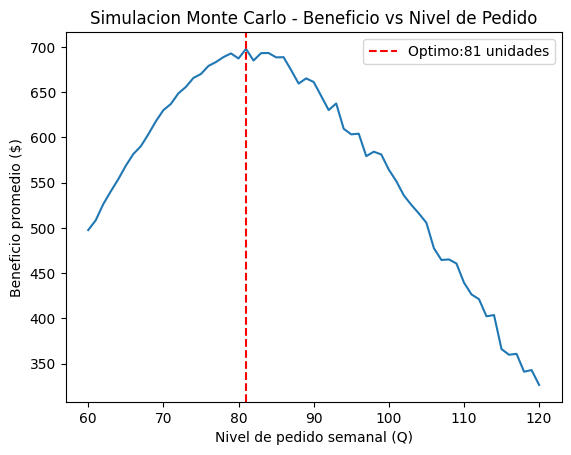
\includegraphics[width=0.7\textwidth]{montecarlo.png}
\end{center}

El nivel de pedido óptimo es el que maximiza el beneficio promedio esperado según la simulación.

\end{document}
